% This tex file is available under a
% Creative Commons Attribution-Share Alike license (CC BY-SA 2.0).
% http://creativecommons.org/licenses/by-sa/2.0/
% Copyright © 2013 Rodrigo Hausen
\documentclass{beamer}
\usepackage[utf8]{inputenc}
\usepackage{lmodern}
\usepackage[T1]{fontenc}
\usepackage[portuguese,brazil]{babel}
\usepackage{url}
\usepackage{listings}
\usepackage{color}
\usepackage{textcomp}
\usepackage{pdfpages}
\usepackage{fancyvrb}
\usepackage{enumerate}
\usepackage{icomma} % para vírgula decimal / decimal comma
\definecolor{listinggray}{gray}{0.9}
\definecolor{lbcolor}{rgb}{0.9,0.9,0.9}
\definecolor{mediumgray}{rgb}{0.6,0.6,0.6}
\lstset{
    backgroundcolor=\color{lbcolor},
    tabsize=4,
    rulecolor=,
    basicstyle=\scriptsize,
    upquote=true,
    aboveskip={1.5\baselineskip},
    columns=fixed,
    showstringspaces=false,
    extendedchars=true,
    breaklines=true,
    prebreak = \raisebox{0ex}[0ex][0ex]{\ensuremath{\hookleftarrow}},
    frame=single,
    showtabs=false,
    showspaces=false,
    showstringspaces=false,
    identifierstyle=\ttfamily,
    keywordstyle=\color[rgb]{0,0,1},
    commentstyle=\color[rgb]{0.133,0.545,0.133},
    stringstyle=\color[rgb]{0.627,0.126,0.941},
}

\definecolor{pinegreen}{RGB}{0,139,114}
\definecolor{pgr}{RGB}{0,139,114}

\definecolor{aquamarine}{RGB}{0,181,190}
\definecolor{aqm}{RGB}{0,181,190}

\definecolor{skyblue}{RGB}{100,227,251}
\definecolor{skb}{RGB}{100,227,251}

\newcommand{\comment}[1]{{\color{structure.fg!70!white}\footnotesize #1}}

\newcommand{\WD}[1]{\fbox{#1}\hspace{-0.5pt}}

\newcommand{\FWD}[1]{%
\fbox{%
\vbox to 10pt{\vfil%
\hbox to 0.8cm{\hfill#1\hfill}%
\vfil}%
}\hspace{-0.5pt}%
}

\def\A{\texttt{A}}
\def\B{\texttt{B}}
\def\C{\texttt{C}}
\def\D{\texttt{D}}
\def\E{\texttt{E}}
\def\F{\texttt{F}}

\usetheme{Boadilla}
%\usetheme{umbc2}
\usefonttheme{structuresmallcapsserif}
\usecolortheme{seahorse}

\title{Aula 5: determinação e simplificação de expressões lógicas}
\subtitle{Circuitos Digitais}
\author{Rodrigo Hausen}
\institute{CMCC -- UFABC} 
\date{4 e 6 de Fev. de 2013}

\input{kmap.tex}

\begin{document}

\begin{frame}
\maketitle

\vspace{-1cm}

\begin{center}
\url{http://compscinet.org/circuitos}
\end{center}

\end{frame}

%%%%%%%%%%%%%%%%%%%%%%%%%%%%%%%%%%%%%%%%%%%%%%%%%

\begin{frame}
 \frametitle{Aula passada: álgebra booleana}

 \textbf{Álgebra booleana} [Boole, 1854]
 \begin{itemize}
 \item Álgebra onde há apenas dois valores válidos: \textbf{falso} e
\textbf{verdadeiro}.
 \item Também denotados:
 \begin{itemize}
   \item \textbf{F} e \textbf{V};
   \item \textbf{false} e \textbf{true} (ou \textbf{F} e \textbf{T});
   \item \textbf{desligado} e \textbf{ligado};
   \item \textbf{0} e \textbf{1}, etc.
 \end{itemize}
 \end{itemize}

\end{frame}

%%%%%%%%%%%%%%%%%%%%%%%%%%%%%%%%%%%%%%%%%%%%%%%%%

\begin{frame}
 \frametitle{Aula passada: operações}

\textbf{Operações}
\begin{itemize}
 \item conjunção (\textbf{e}, \textbf{and}): $X \cdot Y$
 \item disjunção (\textbf{ou}, \textbf{or}: $X + Y$
 \item negação (\textbf{não}, \textbf{not}: $\overline{X}$
 \item disjunção exclusiva (\textbf{ou-ex}, \textbf{xor}): $X \oplus Y =
\overline{X} \cdot Y + X \cdot \overline{Y}$
\end{itemize}

\textbf{Tabelas verdade}.\\[12pt]

\begin{center}

\begin{minipage}{16ex}
\centering
Tabela verdade da conjunção (\textbf{e})\\[6pt]
\begin{tabular}{cc|c}
 $X$ & $Y$ & $X \cdot Y$ \\
\hline
 $0$ & $0$ & $0$ \\
 $0$ & $1$ & $0$ \\
 $1$ & $0$ & $0$ \\
 $1$ & $1$ & $1$
\end{tabular}
\end{minipage}
%
\hspace{3ex}
%
\begin{minipage}{18ex}
\centering
Tabela verdade da disjunção  (\textbf{ou})\\[6pt]
\begin{tabular}{cc|c}
 $X$ & $Y$ & $X + Y$ \\
\hline
 $0$ & $0$ & $0$ \\
 $0$ & $1$ & $1$ \\
 $1$ & $0$ & $1$ \\
 $1$ & $1$ & $1$
\end{tabular}
\end{minipage}
%
\hspace{3ex}
%
\begin{minipage}{18ex}
\centering
Tabela verdade da negação  (\textbf{não})\\[12pt]
\begin{tabular}{c|c}
 $X$ & $\overline{X}$ \\
\hline
 $0$ & $1$ \\
 $1$ & $0$
\end{tabular}
\end{minipage}

\end{center}

\end{frame}


%%%%%%%%%%%%%%%%%%%%%%%%%%%%%%%%%%%%%%%%%%%%%%%%%

\begin{frame}
 \frametitle{Aula passada: expressões e funções lógicas}

\begin{itemize}
\item Expressões lógicas:
  \begin{itemize}
    \item $\overline{1} + (0 \cdot 1)$\\[6pt]
    \item $\overline{X} \cdot Y + X \cdot \overline{Y}$\\[6pt]
    \item $\overline{ A + \overline{B} \cdot C } + A \cdot C + B$
  \end{itemize}
\item Funções lógicas: dadas por uma expressão ou tabela verdade
\vspace{6pt}
  \begin{itemize}
    \item
      \begin{tabular}{cc||c}
      $X$ & $Y$ & $F(X,Y)$ \\
      \hline
      0 & 0 & 0 \\
      0 & 1 & 1 \\
      1 & 0 & 0 \\
      1 & 1 & 1
      \end{tabular}
\vspace{6pt}
    \item $F(X,Y) = \overline{X} \cdot Y + X \cdot Y$
  \end{itemize}
\end{itemize}

\end{frame}

%%%%%%%%%%%%%%%%%%%%%%%%%%%%%%%%%%%%%%%%%%%%%%%%%

\begin{frame}
 \frametitle{Aula passada: regras básicas}

\begin{minipage}[t]{0.34\textwidth}
 1. $X + 0 = X$ \\
\footnotesize{elem. neutro da disjunção}
\end{minipage}
%
\begin{minipage}[t]{0.31\textwidth}
 2. $X+1 = 1$
\end{minipage}
%
\begin{minipage}[t]{0.32\textwidth}
 3. $X + Y = Y + X$ \\
 \footnotesize{comutatividade da disjunção}
\end{minipage}

\vspace{12pt}

\begin{minipage}[t]{0.34\textwidth}
 4. $X \cdot Y = Y \cdot X$\\
 \footnotesize{comutatividade da conjunção}
\end{minipage}
%
\begin{minipage}[t]{0.31\textwidth}
 5. $X + X = X$
\end{minipage}
%
\begin{minipage}[t]{0.32\textwidth}
 6. $X + \overline{X} = 1$
\end{minipage}

\vspace{12pt}

\begin{minipage}[t]{0.34\textwidth}
 7. $X \cdot 0 = 0$
\end{minipage}
%
\begin{minipage}[t]{0.31\textwidth}
 8. $X \cdot 1 = X$ \\
 \footnotesize{elem. neutro da conjunção}
\end{minipage}
%
\begin{minipage}[t]{0.32\textwidth}
 9. $X \cdot X = X$
\end{minipage}

\vspace{12pt}

\begin{minipage}[t]{0.34\textwidth}
 10. $X \cdot \overline{X} = 0$
\end{minipage}
%
\begin{minipage}[t]{0.31\textwidth}
 11. $X \oplus X = 0$ 
\end{minipage}

\vspace{12pt}

\begin{minipage}[t]{0.54\textwidth}
 12. $X + (Y + Z) = (X + Y) + Z$ \\
 \footnotesize{associatividade da disjunção}
\end{minipage}
%
\begin{minipage}[t]{0.34\textwidth}
 13. $X \cdot (Y \cdot Z) = (X \cdot Y) \cdot Z$
 \footnotesize{associatividade da conjunção}
\end{minipage}

\vspace{12pt}

14. $X \cdot (Y + Z) = X \cdot Y + X \cdot Z$ \hspace{1ex}
{\footnotesize{distributividade da conjunção}}

\vspace{6pt}

Leis de Morgan (ou Leis de DeMorgan)

\vspace{6pt}

\begin{minipage}[t]{0.34\textwidth}
 15. $\overline{X + Y} = \overline{X} \cdot \overline{Y}$
\end{minipage}
%
\begin{minipage}[t]{0.31\textwidth}
 16. $\overline{X \cdot Y} = \overline{X} + \overline{Y}$ 
\end{minipage}

\end{frame}

\newcommand{\Not}[1]{\overline{#1}}
\newcommand{\AND}{\cdot}
\newcommand{\OR}{+}
\newcommand{\XOR}{\oplus}
\newcommand{\Mt}[4]{#1 \hspace{-1.5pt} \AND \hspace{-1.5pt} #2 \hspace{-1.5pt}%
\AND \hspace{-1.5pt} #3 \hspace{-1.5pt} \AND #4}

%%%%%%%%%%%%%%%%%%%%%%%%%%%%%%%%%%%%%%%%%%%%%%%%%

\begin{frame}
 \frametitle{Um problema meteorológico}

\textbf{Exemplo 1:} O tempo para o dia seguinte na cidade
de Booleville é bem regular e fácil de prever. O meteorologista
da cidade criou uma tabela para prever se haverá chuva no dia
seguinte (representada pela variável $C$) a partir de quatro
variáveis cujo valor depende das condições meteorológicas do
dia anterior.

\begin{itemize}
\item V -- se está ventando
\item F -- se faz frio
\item U -- se está úmido
\item N -- se está nublado
\end{itemize}

As quatro variáveis são medidas pelo meteorologista e ele
atribui um valor $0$ (falso) ou $1$ (verdadeiro) para cada
uma delas.\\[6pt]

\pause

Ou seja, $C$ é função booleana de $V$, $F$, $U$ e $N$:
$$C = C(V,F,U,N)$$

\end{frame}

%%%%%%%%%%%%%%%%%%%%%%%%%%%%%%%%%%%%%%%%%%%%%%%%%

\begin{frame}
 \frametitle{De tabela verdade para expressão lógica}

Previsão do tempo em Booleville: $C$ (chuva amanhã) função
lógica de\\$V$ (vento hoje), $F$ (frio hoje), $U$ (dia úmido
hoje) e $N$ (nublado hoje).
% Um meteorologista construiu a seguinte tabela a partir da observação das
% condições atmosféricas.

\vspace{6pt}

\begin{tabular}{c@{ }c@{ }c@{ }c||c@{ }l}
 $V$ & $F$ & $U$ & $N$ & $C$ \\
\cline{1-5}
  0  &  0  &  0  &  0  &  0  \\
  0  &  0  &  0  &  1  &  0  \\
  0  &  0  &  1  &  0  &  0  \\
  0  &  0  &  1  &  1  &  1  &
    \uncover<2->{$\longrightarrow \Mt{ \Not{V} }{ \Not{F} }{ U }{ N }$} \\
  0  &  1  &  0  &  0  &  0  \\
  0  &  1  &  0  &  1  &  1  &
    \uncover<3->{$\longrightarrow \Mt{ \Not{V} }{ F }{ \Not{U} }{ N }$} \\
  0  &  1  &  1  &  0  &  1  &
    \uncover<4->{$\longrightarrow \Mt{ \Not{V} }{ F }{ U }{ \Not{N} }$} \\
  0  &  1  &  1  &  1  &  1  &
    \uncover<5->{$\longrightarrow \Mt{ \Not{V} }{ F }{ U }{ N }$}
\end{tabular}
\begin{tabular}{c@{ }c@{ }c@{ }c||cl}
 $V$ & $F$ & $U$ & $N$ & $C$ \\
\cline{1-5}
  1  &  0  &  0  &  0  &  0  \\
  1  &  0  &  0  &  1  &  1  &
    \uncover<5->{$\longrightarrow \Mt{ V }{ \Not{F} }{ \Not{U} }{ N }$} \\
  1  &  0  &  1  &  0  &  1  &
    \uncover<5->{$\longrightarrow \Mt{ V }{ \Not{F} }{ U }{ \Not{N} }$} \\
  1  &  0  &  1  &  1  &  0  \\
  1  &  1  &  0  &  0  &  0  \\
  1  &  1  &  0  &  1  &  0  \\
  1  &  1  &  1  &  0  &  1  &
    \uncover<5->{$\longrightarrow \Mt{ V }{ F }{ \Not{U} }{ N }$} \\
  1  &  1  &  1  &  1  &  1  &
    \uncover<5->{$\longrightarrow \Mt{ V }{ F }{ U }{ N }$}
\end{tabular}

\uncover<6->{
\vspace{6pt}

\begin{eqnarray*}
 C(V,F,U,N) & = & \Mt{ \Not{V} }{ \Not{F} }{ U }{ N } +
\pause\pause\pause\pause\pause\pause
              \Mt{ \Not{V} }{ F }{ \Not{U} }{ N } +
\pause
              \Mt{ \Not{V} }{ F }{ U }{ \Not{N} } +
\pause
              \Mt{ \Not{V} }{ F }{ U }{ N } + \\
\pause
            & + &
	      \mbox{$\Mt{ V }{ \Not{F} }{ \Not{U} }{ N }$} +
              \Mt{ V }{ \Not{F} }{ U }{ \Not{N} } +
              \Mt{ V }{ F }{ \Not{U} }{ N } +
              \Mt{ V }{ F }{ U }{ N }
\end{eqnarray*}
}

\end{frame}

%%%%%%%%%%%%%%%%%%%%%%%%%%%%%%%%%%%%%%%%%%%%%%%%%

\def\And{\,}

\begin{frame}
 \frametitle{De tabela verdade para expressão lógica}

Para facilitar a escrita, quando escrevemos uma conjunção,
podemos considerar que o sinal ``$\cdot$'' está implícito,
como fazemos na álgebra comum.\\[-6pt] 

\begin{eqnarray*}
 C(V,F,U,N) & = & \Not{V} \And \Not{F} \And U       \And N +
                  \Not{V} \And F       \And \Not{U} \And N +
                  \Not{V} \And F       \And U       \And \Not{N} +
                  \Not{V} \And F       \And U       \And N +\\
            & + &
	          V \And \Not{F} \And \Not{U} \And N +
                  V \And \Not{F} \And U       \And \Not{N} +
                  V \And F       \And \Not{U} \And N +
                  V \And F       \And U       \And N
\end{eqnarray*}

\pause

Vamos simplificar essa expressão. Colocando em evidência:

\begin{eqnarray*}
C(V,F,U,N) & = & \Not{V} N \And ( \Not{F} \And U + F \And \Not{U} ) +
                 \Not{V} \And F \And U \And ( \Not{N} + N ) +\\
           & + & V \And \Not{F} \And ( \Not{U} \And N + U \And \Not{N} ) +
                 V \And F \And N \And ( \Not{U} + U )
\end{eqnarray*}

\pause

Usando a definição do \textbf{xor}
$X \oplus Y = \Not{X} \And Y + X \And \Not{Y}$ e as regras
 $\Not{X} + X = 1$ e $X \AND 1 = X$:

\vspace{6pt}

$C(V,F,U,N) = \Not{V} \And N \And ( F \XOR U ) +
              \Not{V} \And F \And U +
              V \And \Not{F} \And ( U \XOR N ) +
              V \And F \And N
$

\pause

\vspace{6pt}

Poderíamos continuar a simplificação. Note que nem sempre é fácil simplificar,
e que outras expressões (equivalentes) são possíveis.

\end{frame}

%%%%%%%%%%%%%%%%%%%%%%%%%%%%%%%%%%%%%%%%%%%%%%%%%

\begin{frame}[fragile]
 \frametitle{Observações sobre funções}

\small
%
 Procedimento para transformar a tabela verdade de uma função
$F(X_1, X_2, \ldots, X_n)$ em expressão lógica:\\[6pt]

\texttt{PARA CADA linha da tabela onde} \(F(X\sb{1}, X\sb{2}, \ldots, X\sb{n})=1\)\\
\hspace{4ex}\texttt{escreva a conjunção \(Y\sb{1}Y\sb{2} \ldots Y\sb{n}\) onde \(Y\sb{i}=\left\{\begin{array}{l}X\sb{i} \text{ se } X\sb{i}=1\\{}\overline{X\sb{i}} \text{ se } X\sb{i}=0\end{array}\right.\)}\\
\texttt{faça a disjunção das conjunções obtidas}\\[6pt]

\pause

Cada uma das conjunções $Y_{1} Y_{2} \ldots Y_{n}$ é chamada \emph{produto de variáveis lógicas} ou \emph{mintermo}.

\vspace{6pt}

Note que o procedimento funciona para \textbf{qualquer} função lógica e a
expressão obtida terá tabela verdade idêntica à da função original.

\pause

\vspace{6pt}

\textbf{Teorema.} Toda função lógica pode ser escrita como disjunção de mintermos (também chamada ``soma de produtos'' -- SOP).\\
Portanto, \textbf{toda função lógica possui uma expressão que a define}.

\pause

\vspace{6pt}

A forma de soma de produtos é uma \textbf{forma padrão} de representação de expressões booleanas. \comment{Outra forma padrão é o \emph{produto de somas}.}

\end{frame}

%%%%%%%%%%%%%%%%%%%%%%%%%%%%%%%%%%%%%%%%%%%%%%%%%
\begin{frame}
\frametitle{Simplificação na forma soma-de-produtos}

É possível simplificar a expressão obtida para $C$ mantendo-a
como soma-de-produtos?

\vspace{6pt}

Observe que:
\begin{eqnarray*}
&   & \Not{V} \And F \And U \And \Not{N} + \Not{V} \And F \And U \And N +
      V \And F \And U \And \Not{N} + V \And F \And U \And N\\ \pause
& = & F \And U \And [ \Not{V} \And \Not{N} + \Not{V} \And N + V \Not{N} + V \And N ] \\ \pause
& = & F \And U \And [ \Not{V} \And ( \Not{N} + N ) + V \And ( \Not{N} + N ) ] \\ \pause
& = & F \And U \And [ \Not{V} + V ] \\ \pause
& = & F \And U \pause
\end{eqnarray*}

Logo, temos uma expressão mais simples para $C$:
$$C = \Not{V} \And \Not{F} \And U \And N + \Not{V} \And F \And \Not{U} \And N +
V \And \Not{F} \And \Not{U} \And N + V \And \Not{F} \And U \And N + F \And U$$

Esta é a menor expressão como soma-de-produtos?
\end{frame}

%%%%%%%%%%%%%%%%%%%%%%%%%%%%%%%%%%%%%%%%%%%%%%%%%
\begin{frame}
\frametitle{Simplificação na forma soma-de-produtos}

Observe que, quando temos algo do tipo:
$$
\ldots + A \And \Not{B} + A \And B + \ldots
$$
em uma expressão na forma soma-de-produtos podemos
colocar $A$ em evidência:
$$
\ldots + A \And ( \Not{B} + B ) + \ldots
$$
e simplificar por:
$$
\ldots + A + \ldots
$$

\vspace{6pt} \pause

\textbf{Problema:} como encontrar dois mintermos idênticos
a menos de uma mesma variável $B$, que aparece como
$B$ e $\Not{B}$?

\vspace{6pt} \pause

\textbf{Solução:} expresse a tabela verdade de forma que
isso seja fácil de encontrar!
\end{frame}

\def\Zero{\raisebox{0pt}{\color{structure.fg!70!white}0}}

%%%%%%%%%%%%%%%%%%%%%%%%%%%%%%%%%%%%%%%%%%%%%%%%%
\begin{frame}
\frametitle{Mapa de Karnaugh}

\small

\hspace*{\fill}
\begin{minipage}{10ex}
Tabela Verdade:
\end{minipage}
\hspace{2ex}
\begin{tabular}{c@{ }c@{ }c@{ }c||c@{ }l}
 $V$ & $F$ & $U$ & $N$ & $C$ \\
\cline{1-5}
  0  &  0  &  0  &  0  &  \Zero  \\
  0  &  0  &  0  &  1  &  \Zero  \\
  0  &  0  &  1  &  0  &  \Zero  \\
  0  &  0  &  1  &  1  &  1  \\
  0  &  1  &  0  &  0  &  \Zero  \\
  0  &  1  &  0  &  1  &  1  \\
  0  &  1  &  1  &  0  &  1  \\
  0  &  1  &  1  &  1  &  1  \\
\end{tabular}
\hspace{4ex}
\begin{tabular}{c@{ }c@{ }c@{ }c||cl}
 $V$ & $F$ & $U$ & $N$ & $C$ \\
\cline{1-5}
  1  &  0  &  0  &  0  &  \Zero  \\
  1  &  0  &  0  &  1  &  1  \\
  1  &  0  &  1  &  0  &  1  \\
  1  &  0  &  1  &  1  &  \Zero  \\
  1  &  1  &  0  &  0  &  \Zero  \\
  1  &  1  &  0  &  1  &  \Zero  \\
  1  &  1  &  1  &  0  &  1  \\
  1  &  1  &  1  &  1  &  1  \\
\end{tabular}
\hspace*{\fill}

\vspace{3pt} \pause


\hspace*{\fill}
\begin{minipage}{20ex}
Mapa de Karnaugh:
outra representação
para a tabela verdade
\end{minipage}
\hspace{2ex}
\begin{kmap}{5}%
\begin{picture}(0,0)\put(-3,15){\line(1,-1){23}}\end{picture}%
\hbox to 3pt{\raisebox{-8pt}{\footnotesize$VF$}}%
\raisebox{8pt}{\footnotesize$UN$}%
      & $00$ & $01$ & $11$ & $10$ \nl
 $00$  &  \Zero   &  \Zero   &  1       &   \Zero  \nl
 $01$  &  \Zero   &  1       &  1       &   1  \nl
 $11$  &  \Zero   &  \Zero   &  1       &   1  \nl
 $10$  &  \Zero   &  1       &  \Zero   &   1  \nl
\end{kmap}
\hspace*{\fill}

\end{frame}

%%%%%%%%%%%%%%%%%%%%%%%%%%%%%%%%%%%%%%%%%%%%%%%%%
\begin{frame}
\frametitle{Mapa de Karnaugh}

Representação em matriz para a tabela verade, onde
\textbf{em linhas ou colunas adjacentes apenas uma
variável muda} de $1$ para $0$ ou vice-versa.

\vspace{6pt}

\hspace*{\fill}%
\only<01>{\includegraphics{images/kmap01_01}}%
\only<02>{\includegraphics{images/kmap01_02}}%
\only<03>{\includegraphics{images/kmap01_03}}%
\only<04>{\includegraphics{images/kmap01_04}}%
\only<05>{\includegraphics{images/kmap01_05}}%
\only<06>{\includegraphics{images/kmap01_06}}%
\only<07>{\includegraphics{images/kmap01_07}}%
\only<08>{\includegraphics{images/kmap01_08}}%
\only<09>{\includegraphics{images/kmap01_09}}%
\only<10>{\includegraphics{images/kmap01_10}}%
\only<11-12>{\includegraphics{images/kmap01_11}}%
\only<13-14>{\includegraphics{images/kmap01_13}}%
\only<15-16>{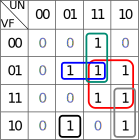
\includegraphics{images/kmap01_15}}%
\hspace*{\fill}

\vspace{6pt}

$C \phantom{\Not{V}} = \phantom{\Not{V}} % phantoms are needed
                                         % to preserve line height
 \only<1-2>{{\color{red} \Not{V} \And F \And U \And N + }}
 \only<2>{{\color{red} \Not{V} \And F \And U \And \Not{N} + }}
 \only<3-6>{{\color{red} \Not{V} \And F \And U + }}
 \only<4-5>{{\color{red} V \And F \And U \And N + }}
 \only<5>{{\color{red} V \And F \And U \And \Not{N} } + }
 \only<6>{{\color{red} V \And F \And U } + }
 \only<7->{{\color{red} F \And U } + }
 \only<8-9>{{\color{blue} \Not{V} \And F \And \Not{U} \And N +} }
 \only<9>{{\color{blue} \Not{V} \And F \And U \And N} + }
 \only<10->{{\color{blue} \Not{V} \And F \And N} + }
 \only<12->{{\color{pinegreen} \Not{V} \And U \And N} + }
 \only<14->{{\color{gray} V \And U \And \Not{N}} + }
 \only<16->{ V \And \Not{F} \And \Not{U} \And N }
$
\end{frame}

%%%%%%%%%%%%%%%%%%%%%%%%%%%%%%%%%%%%%%%%%%%%%%%%%
\begin{frame}
\frametitle{Mapa de Karnaugh}

\textbf{Exemplo 2: } Simplifique
\begin{eqnarray*}
F(A,B,C,D) & = & \Not{A} \And \Not{B} \And \Not{C} \And \Not{D} +
                 A \And \Not{B} \And C \And \Not{D} +
                 A \And \Not{B} \And \Not{C} \And D +
                 \Not{A} \And \Not{B} \And C \And D +\\
           & + & A \And \Not{B} \And \Not{C} \And \Not{D} +
                 \Not{A} \And \Not{B} \And \Not{C} \And D +
                 \Not{A} \And \Not{B} \And C \And \Not{D} +
                 A \And \Not{B} \And C \And D
\end{eqnarray*}

\hspace*{\fill}%
\only<1>{\includegraphics{images/kmap02_00}}%
\only<2>{\includegraphics{images/kmap02_01}}%
\only<3->{\includegraphics{images/kmap02_02}}%
\hspace*{\fill}

\uncover<4->{
$$
	F(A,B,C,D) = {\color{red}\Not{A} \And \Not{B}} + A \And \Not{B}
\uncover<5->{ = (\Not{A} + A) \And B }
\uncover<6->{ = B }
$$
}

\vspace{-20pt}

\uncover<7->{
Será que poderíamos observar a última simplificação no mapa?
}

\end{frame}

%%%%%%%%%%%%%%%%%%%%%%%%%%%%%%%%%%%%%%%%%%%%%%%%%
\begin{frame}
\frametitle{Mapa de Karnaugh}

Como a exigência é que apenas uma variável mude entre linhas/colunas
adjacentes, poderíamos ter feito o mapa como:

\vspace{8pt}

\hspace*{\fill}%
\only<1>{\includegraphics{images/kmap03_01}}%
\only<2->{\includegraphics{images/kmap03_02}}%
\hspace*{\fill}

\vspace{8pt}

\pause\pause

A única variável que não mudou foi \pause $B$, que permaneceu em $0$\pause,
portanto $F(A,B,C,D) = \Not{B}$.

\end{frame}

%%%%%%%%%%%%%%%%%%%%%%%%%%%%%%%%%%%%%%%%%%%%%%%%%
\begin{frame}
\frametitle{Mapa de Karnaugh}

Podemos ver essa simplificação diretamente no mapa original,
se considerarmos que \textbf{a última linha é adjacente à
primeira linha}, assim como \textbf{a última coluna é adjacente à
primeira coluna}.

\pause

\vspace{12pt}

\hspace*{\fill}%
\only<1>{\includegraphics{images/kmap04_00}}%
\only<2>{\includegraphics{images/kmap04_01}}%
\only<3->{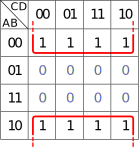
\includegraphics{images/kmap04_02}}%
\hspace*{\fill}

\pause\pause

$$F(A,B,C,D) = \Not{B}$$

\end{frame}

%%%%%%%%%%%%%%%%%%%%%%%%%%%%%%%%%%%%%%%%%%%%%%%%%
\begin{frame}
\frametitle{Mapa de Karnaugh: como usar}

\small

Para até $4$ variáveis:

\begin{itemize}
\item 1. Expresse a tabela verdade como uma matriz, com no máximo
duas variáveis para as linhas/colunas. Em linhas adjacentes,
apenas uma das variáveis muda (o mesmo vale para as colunas).\\
\comment{Sugestão de rótulos para as linhas/colunas: 00, 01, 11, 10}
\pause
\item 2. Enquanto houver uma célula contendo $1$ que não tiver sido
agrupada, agrupe nesta ordem:
\begin{enumerate}
\item Retângulos com 16 uns (\textbf{Obs.:} se houver, então $F = 1$)
\pause
\item Retângulos com 8 uns (2x4 ou 4x2)
\pause
\item Retângulos com 4 uns (1x4, 4x1 ou 2x2)
\pause
\item Retângulos com 2 uns (1x2 ou 2x1)
\pause
\item Retângulos com apenas 1 um
\pause
\end{enumerate}
\textbf{Importante: } a última linha/coluna é adjacente à primeira linha/coluna.
\pause
\item 3. Elimine grupos redundantes (se puder)
\pause
\item 4. Para cada grupo, escreva uma soma de produtos onde apenas as
variáveis que não mudaram são representadas. \textbf{Importante: } 
Se, no grupo, uma variável $X$ é mantida em $0$, então escreva $\Not{X}$.
\end{itemize}
\end{frame}

%%%%%%%%%%%%%%%%%%%%%%%%%%%%%%%%%%%%%%%%%%%%%%%%%
\begin{frame}
\frametitle{Mapa de Karnaugh: Exemplos}

\begin{minipage}{38ex}
\raggedright
\textbf{Exemplo 3: } Simplifique $F(A,B,C,D)$,
cuja tabela verdade é dada pelo mapa de Karnaugh
ao lado.\\[24pt]
\uncover<2->{
Resp.: $F = \Not{A} \, \Not{C} + \Not{A} \, B + A \, \Not{B} \, D$
}
\end{minipage}
\begin{minipage}{30ex}
\includegraphics{images/kmap05}
\end{minipage}

\vspace{12pt}\pause\pause

\textbf{Exemplo 4: } Simplifique $\Not{A} \And \Not{B} \And \Not{C} + \Not{A} \And \Not{B} \And C + A \And B \And \Not{C} + A \And \Not{B} \And \Not{C}$

\vspace{12pt}\pause

\textbf{Exemplo 5: } Simplifique $\Not{A} \And \Not{B} \And C + \Not{A} \And B \And \Not{C} + A \And B \And \Not{C} + A \And B \And C$

\vspace{12pt}\pause

\textbf{Exemplo 6: } Simplifique $A \, B \, C \, D  +
A \, B \, \Not{C} \, D  +  A \, B \, \Not{C} \, \Not{D}  +
A \, \Not{B} \, C \, D  +  \Not{A} \, B \, C \, D  +
\Not{A} \, B \, C \, \Not{D} + \Not{A} \, B \, \Not{C} \, D  +
\Not{A} \, \Not{B} \, \Not{C} \, D$
\end{frame}

%%%%%%%%%%%%%%%%%%%%%%%%%%%%%%%%%%%%%%%%%%%%%%%%%
\begin{frame}
\frametitle{Mais de 4 variáveis}

\small

É possível construir mapas de Karnaugh para mais de $4$ variáveis,
mas eles se tornam difíceis de representar.

\vspace{6pt}\pause

Para 6 variáveis, o mapa torna-se um cubo:

\vspace{6pt}

{\centering
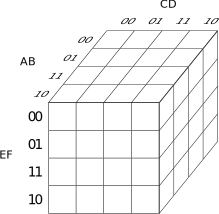
\includegraphics[scale=0.7]{images/kmap6var}\\}

\vspace{6pt}\pause

Entre $4$ e $30$ (aprox.) variáveis, é possível executar
o \textbf{método de Quine-McCluskey}, que é exato mas possui
complexidade exponencial.\\ \pause
Acima de $30$ variáveis, há o minimizador
\textbf{Espresso}, baseado em métodos heurísticos (não exato).

\end{frame}

%%%%%%%%%%%%%%%%%%%%%%%%%%%%%%%%%%%%%%%%%%%%%%%%%
\begin{frame}
\frametitle{Conclusão}

O mapa de Karnaugh é um método de representar a tabela verdade
de uma função lógica de tal modo que os termos de uma soma-de-produtos
que podem ser simplificados estão sempre adjacentes.

\vspace{6pt}

\textbf{Importante: } Recomenda-se colocar as linhas/colunas nesta
ordem:\\00, 01, 11, 10. Sempre troque \textbf{apenas uma} variável
a cada linha/coluna.

\vspace{6pt} \pause

Mapas de Karnaugh são fáceis de se usar para até $4$ variáveis. \pause Para
$5$ e $6$ variáveis, é possível:
\begin{itemize}
\item Simplificar algebricamente, até obtermos $4$ variáveis, e
depois usar o mapa de Karnaugh.
\begin{itemize}
\item Exemplo: simplifique $A \, B \, C \, D \, E +
A \, B \, \Not{C} \, D \, E  +  A \, B \, \Not{C} \, \Not{D} \, E  +
A \, \Not{B} \, C \, D \, E +  \Not{A} \, B \, C \, D \, E  +
\Not{A} \, B \, C \, \Not{D} \, E + \Not{A} \, B \, \Not{C} \, D \, E  +
\Not{A} \, \Not{B} \, \Not{C} \, D \, E$
\end{itemize}
\pause
\item Ou usar mapas de Karnaugh tridimensionais.
\end{itemize}

\vspace{6pt} \pause

A partir de $4$ variáveis, costuma ser mais vantajoso usar outros métodos
(Quine-McCluskey ou Espresso).

\end{frame}

%%%%%%%%%%%%%%%%%%%%%%%%%%%%%%%%%%%%%%%%%%%%%%%%%
\begin{frame}
\frametitle{Para casa:}

\begin{itemize}
\item Ler seções 4-6, 4-7, 4-8, 4-9 e o final do capítulo intitulado
``Aplicações em sistemas digitais'' (desprezar os comentários e diagramas
sobre portas lógicas; nós veremos portas lógicas na próxima aula).
\item Exercícios recomendados:
\begin{itemize}
\item Autotestes: 12 a 16
\item Problemas: 21 a 44
\end{itemize}
\end{itemize}
\end{frame}

\end{document}
